\documentclass[12pt,prb,aps]{revtex4-1}
\usepackage {amsmath}
\usepackage{amssymb}
\pdfoutput = 1 
\usepackage {graphicx}
\newcommand{\bomega}{\mbox{\boldmath$\omega$}}
\allowdisplaybreaks

\begin{document}

\title{Time-Dependent Parallel Electron Energy Transport in  a Magnetized Plasma of Arbitrary Collisionality}
\author{T.~Wang\,\footnote{wt@utexas.edu} and R.~Fitzpatrick}
\affiliation{Institute for Fusion Studies,  Department of Physics,  University of Texas at Austin,  Austin TX 78712, USA}

\begin{abstract}
The analysis of Hazeltine [Phys.\ Plasmas {\bf 5}, 3282 (1998)], which considers the transport of electron number density and energy parallel to the magnetic
field in a magnetized plasma of arbitrary collisionality,  is generalized by  incorporating a model electron-ion collision operator,
 including a self-consistent calculation of the parallel electric field, and taking time dependence into account. The resulting enhanced model is
 used to investigate the transport of electron energy across a magnetic island chain in a tokamak plasma. A general expression for the critical
 island width above which the electron temperature profile is flattened inside the magnetic separatrix of the island chain is derived.
 This expression is valid at arbitrary electron collisionality, and also allows for temporal oscillation of the radial temperature gradient across the island chain. 
 The expression is shown to asymptote to much  simpler expressions in the short mean-free-path and long mean-free-path limits. An expression for
 the appropriate value of the parallel electron thermal conductivity to use in extended magnetohydrodynamical simulation codes that represent parallel
 electron energy transport in terms of a diffusive operator is obtained. 
 \end{abstract}
\maketitle

\section{Introduction}
In Hazeltine (1998),\cite{haz}  the steady-state transport of electron number density and energy parallel to the magnetic field
of a magnetized, weakly-coupled, electron-ion plasma of arbitrary collisionality is investigated  in slab geometry   by solving a simplified one-dimensional kinetic equation for the electron distribution function that employs a Bhatnagar-Gross-Krook (BGK)  electron-electron collision
operator.\cite{krook}  The resulting model is able to successfully reproduce standard results for the the electron heat flux in both the short mean-free-path and
the long mean-free-path limits. In the short mean-free-path limit, electron energy transport is found to be local and diffusive in nature, whereas the transport is found to be non-local and convective in the
long mean-free-path limit. 

The aim of this paper is to generalize the analysis of Hazeltine (1998) by  incorporating a model electron-ion collision operator,
 including a self-consistent calculation of the parallel electric field, and taking time dependence into account. The resulting enhanced model is used to investigate the transport of electron
 energy across a magnetic island chain in a tokamak plasma. 

\section{Fundamental Model}\label{s2}

\subsection{Electron Distribution Function}
Let $f_e(t,{\bf x},{\bf v})$ be the ensemble-averaged electron distribution function. Here, $t$ denotes time, ${\bf x}=(x_1,\, x_2,\, x_3)$
is a position vector,  $x_1$, $x_2$, $x_3$ are Cartesian coordinates that are defined such that the 
$x_3$-axis is parallel to the local equilibrium magnetic field, and ${\bf v}$ is the electron velocity. 
Let us write
\begin{equation}\label{e22}
f_e(t,{\bf x},{\bf v})= n_e\,F(v_1)\,F(v_2)\left[F(v_3)+ f (t,x_3,v_3)\right],
\end{equation}
where 
\begin{equation}
F(v) = \frac{\exp(-v^2/v_{t\,e}^{\,2})}{\pi^{1/2}\,v_{t\,e}},
\end{equation}
and 
$|f/F|\ll 1$. Here,  $n_e$ is the unperturbed electron number density, 
\begin{equation}\label{vte}
v_{t\,e} = \sqrt{\frac{2\,T_e}{m_e}}
\end{equation}
the electron thermal velocity, $m_e$  the electron mass,  and $T_e$ the unperturbed electron temperature (measured in energy units). Note that we are assuming that the electron distribution function remains relatively close to a Maxwellian distribution. 

\subsection{Electron-Electron Collision Operator}\label{see}
The electron-electron collision operator is modeled as a BGK operator:\,\cite{haz,krook}
\begin{align}
C_{ee}(f_e) &= -\nu_{ee}\,F(v_1)\,F(v_2)\,\biggr\{n_e\,F(v_3)+n_e\,f(t,x_3,v_3)\phantom{\frac{a}{b}}\nonumber\\[0.5ex]
&\phantom{=}\left.- \frac{[n_e+\delta n_e(t,x_3)]\,m_e^{\,1/2}}{\pi^{1/2}\,(2\,[T_e+\delta T_e(t,x_3)])^{1/2}}\,\exp\left[-\frac{[v_3-V_e(t,x_3)]^{2}\,m_e}{2\,[T_e+\delta T_e(t,x_3)]}\right]\right\}.
\end{align}
Here, $\nu_{ee}$ is the electron-electron collision frequency. Moreover, $|\delta n_e/n_e|\ll 1$, $|V_e/v_3|\ll 1$,  and $|\delta T_e/T_e|\ll 1$. It can be seen that the operator acts to relax the distribution function to the 
perturbed Maxwellian
\begin{equation}
F(v_1)\,F(v_2)\,\frac{[n_e+\delta n_e(t,x_3)]\,m_e^{\,1/2}}{\pi^{1/2}\,(2\,[T_e+\delta T_e(t,x_3)])^{1/2}}\,\exp\left[-\frac{[v_3-V_3(t,x_3)]^{2}\,m_e}{2\,[T_e+\delta T_e(t,x_3)]}\right].
\end{equation}
Note that we are working in an assumed common electron-ion rest frame.
Expanding the collision operator, and only retaining terms that are first order in perturbed quantities, we obtain
\begin{align}\label{e24}
C_{ee}(f_e) &=- \nu_{ee}\,n_e\,F(v_1)\,F(v_2)\,\left\{ f(t,x_3,v_3) - \left[\frac{\delta n_e(t,x_3)}{n_e} +\frac{V_e(t,x_3)}{v_{t\,e}} \,\frac{2\,v_3}{v_{t\,e}}\right.\right.\nonumber\\[0.5ex]
&\phantom{=}\left.\left.+\frac{\delta T_e(t,x_3)}{T_e}\left(\frac{v_3^{\,2}}{v_{t\,e}^{\,2}}-\frac{1}{2}\right)\right]F(v_3)\right\}.
\end{align}

Now, in order for the electron-electron collision operator to conserve the number of electrons, we require that
\begin{equation}
\int\!\!\int\!\!\int C_{ee}(f_e) \,d^3{\bf v} = 0,
\end{equation}
which yields
\begin{equation}\label{dne}
\frac{\delta n_e(t,x_3)}{n_e} =\int_{-\infty}^\infty f(t,x_3,v_3)\,dv_3.
\end{equation}
Here, $\delta n_e(t,x_3)$ is the perturbed electron number density. 

Likewise, in order for the electron-electron collision operator to conserve electron momentum, we need
\begin{equation}\label{e27}
\int\!\!\int\!\!\int {\bf v}\,C_{ee}(f_e)\, d^3{\bf v}= {\bf 0}.
\end{equation}
It is easily seen that 
$\int\!\!\int\!\!\int v_1\,C_{ee}(f_e)\,d^3{\bf v} =\int\!\!\int\!\!\int v_2\,C_{ee}(f_e)\,d^3{\bf v} = 0$.
Thus, we require 
\begin{equation}\label{eyy}
\int\!\!\int\!\!\int v_3\,C_{ee}(f_e)\, d^3{\bf v} = 0,
\end{equation}
which yields
\begin{equation}\label{e29}
 V_e(t,x_3) = \int_{-\infty}^\infty v_3\,f(t,x_3,v_3)\,dv_3.
\end{equation}
Here, $V_e(t,x_3)$ is the perturbed parallel drift velocity of the electrons with respect to the ions.

Finally, in order for the electron-electron collision operator to conserve electron energy, we require
\begin{equation}\label{e20}
\int\!\!\int\!\!\int v^2\,C_{ee}(f_e)\, d^3{\bf v} = 0.
\end{equation}
It is easily seen that 
$\int\!\!\int\!\!\int v_1^{\,2}\,C_{ee}(f_e) \,d^3{\bf v} = \int\!\!\int\!\!\int v_2^{\,2}\,C_{ee}(f_e)\,d^3{\bf v} =0$.
Thus, we need 
\begin{equation}\label{e36s}
\int\!\!\int\!\!\int v_3^{\,2}\,C_{ee}(f_e) \,d^3{\bf v} = 0,
\end{equation}
which yields
\begin{equation}\label{dte}
\frac{\delta T_e(t,x_3)}{T_e} = 2\,\int_{-\infty}^\infty \left(\frac{v_3^{\,2}}{v_{t\,e}^{\,2}}-\frac{1}{2}\right) f(t,x_3,v_3)\,dv_3.
\end{equation}
Here, $\delta T_e(t,x_3)$ is the perturbed electron temperature.
Thus, the electron-electron collision operator, (\ref{e24}), is now fully specified in terms of the perturbed electron distribution function,
$f(t,x_3,v_3)$. 

\subsection{Electron-Ion Collision Operator}
By analogy with the analysis in the previous subsection, our model electron-ion collision operator is written
\begin{align}
C_{ei}(f_e) &=- \nu_{ei}\,n_e\,F(v_1)\,F(v_2)\,\biggr\{ f(t,x_3,v_3) \nonumber\\[0.5ex]&\phantom{=}\left.- \left[\frac{\delta n_e(t,x_3)}{n_e} +\frac{\delta T_e(t,x_3)}{T_e}\,\left(\frac{v_3^{\,2}}{v_{t\,e}^{\,2}}-\frac{1}{2}\right)\right]F(v_3)\right\},
\end{align}
where $\nu_{ei}$ is the electron-ion collision frequency. Note that this collision operator conserves the number of electrons, as well as the electron energy (because the ions are treated as
infinitely massive with respect to the electrons), but does not conserve electron momentum (as a consequence of momentum transferred to the ions via collisions). Note, finally, that the
ion fluid is stationary in the infinite mass limit. 

\subsection{Electron Kinetic Equation}
The  ensemble-averaged electron kinetic equation that governs the transport of electron number density
and energy parallel to the magnetic field can be written\,\cite{haz,rf0}
\begin{equation}
\frac{\partial f_e}{\partial t}+v_3\,\frac{\partial f_e}{\partial x_3} -\frac{e}{m_e}\,E_3\,\frac{\partial f_e}{\partial v_3} = C_{ei}(f_e) + C_{ee}(f_e) + S({\bf x},{\bf v}).
\end{equation}
Here, we are assuming that the plasma is subject to a perturbed parallel electric
field, $E_3(t,x_3)$. Moreover, the source term in the kinetic equation takes the form 
\begin{equation}
S(t,{\bf x},{\bf v}) = n_e\,F(v_1)\,F(v_2)\,F(v_3)\left[S_0(t,x_3) +S_2(t,x_3)\left(\frac{v_3^{\,2}}{v_{t\,e}^{\,2}}-\frac{1}{2}\right) \right],
\end{equation}
where $S_0(t,x_3)$ represents a particle source, and $S_2(t,x_3)$ represents an energy source. 

Linearizing the kinetic equation, and integrating over $v_1$ and $v_2$, we obtain
\begin{equation}\label{e40}
\frac{\partial f}{\partial t}+v_3\,\frac{\partial f}{\partial x_3} - \langle C_{ei}( f)\rangle- \langle C_{ee}(f)\rangle = \left[
S_0 +S_1\,\frac{2\,v_3}{v_{t\,e}} +S_2 \left(\frac{v_3^{\,2}}{v_{t\,e}^{\,2}}-\frac{1}{2}\right)\right]F(v_3),
\end{equation}
where
\begin{align}\label{cee}
\langle C_{ee}(f)\rangle&= \frac{1}{n_e}\int_{-\infty}^\infty\!\int_{-\infty}^\infty C_{ee}(f_e)\,dv_1\,dv_2\nonumber\\[0.5ex]&= -\nu_{ee}\left\{f-\left[\frac{\delta n_e}{n_e}+\frac{ V_e}{v_{t\,e}}\,\frac{2\,v_3}{v_{t\,e}}
+\frac{\delta T_e}{T_e}\left(\frac{v_3^{\,2}}{v_{t\,e}^{\,2}}-\frac{1}{2}\right)\right]F(v_3)\right\},\\[0.5ex]
\langle C_{ei}(f)\rangle&= \frac{1}{n_e}\int_{-\infty}^\infty\!\int_{-\infty}^\infty C_{ei}(f_e)\,dv_1\,dv_2\nonumber\\[0.5ex]&=-\nu_{ei}\left\{f-\left[\frac{\delta n_e}{n_e}
+\frac{\delta T_e}{T_e}\left(\frac{v_3^{\,2}}{v_{t\,e}^{\,2}}-\frac{1}{2}\right)\right]F(v_3)\right\},\label{cei}\\[0.5ex]
S_1(t,x_3) &= - \frac{e\, E_3(t,x_3)}{m_e\,v_{t\,e}}.\label{s1}
\end{align}

\subsection{Poisson-Maxwell Equation}
Assuming that the ions constitute a uniform neutralizing background, the perturbed parallel electric field is related to the perturbed electron number
density according to
\begin{equation}\label{pois}
\frac{\partial  E_3}{\partial x_3}=-\frac{e\,\delta n_e(t,x_3)}{\epsilon_0}.
\end{equation}

\subsection{Heat Flux}
The flux of parallel electron kinetic energy is defined\,\cite{rf0}
\begin{equation}
{\bf q}_\parallel(t,{\bf x}) =  \int\!\int\!\int \frac{1}{2}\,m_e\,(v_3-V_e)^2\,({\bf v}-{\bf V})\,f_e(t,{\bf x},{\bf v})\,d^3{\bf v}.
\end{equation}
It is easily demonstrated that, to first order in small quantities, $q_{\parallel\,1}=q_{\parallel\,2}=0$, and
\begin{equation}\label{q3}
q_{\parallel\,3}(t,x_3) = \frac{1}{2}\,m_e\,n_e\int_{-\infty}^\infty v_3\left(v_3^{\,2}
-\frac{3}{2}\,v_{t\,e}^{\,2}\right)f(t,x_3,v_3)\,dv_3.
\end{equation}

\section{Fourier-Laplace Transform Solution of Electron Kinetic Equation}\label{s3}
\subsection{Normalization}
Let
\begin{align}\label{enu}
\nu_e= \nu_{ee}+\nu_{ei}
\end{align}
be the total electron collision frequency, and
let
\begin{equation}\label{el}
l_e= \frac{v_{t\,e}}{\nu_e}
\end{equation}
be the electron mean-free-path between collisions. 
Let us adopt the following normalizations: 
$\hat{t} = \nu_{e}\,t$,
$\hat{x}= x_3/l_e$,
$u = v_3/v_{t\,e}$,
$\hat{f}= v_{t\,e}\,f$,
$\delta\hat{n}_e= \delta n_e/n_e$,
$\hat{V}_e= V_e/v_{t\,e}$,
$\delta\hat{T}_e= \delta T_e/T_e$,
$\hat{S}_0 = S_0/\nu_{e}$,
$\hat{S}_1 = S_1/\nu_{e}$,
$\hat{S}_2= S_2/\nu_{e}$, and
$\hat{q}_e=q_{\parallel\,3}/(n_e\,T_e\,v_{t\,e})$.
 
The electron kinetic equation, (\ref{e40}), takes the normalized form
\begin{align}\label{e37a}
\frac{\partial\hat{f}}{\partial \hat{t}}+u\,\frac{\partial\hat{f}}{\partial\hat{x}} + \hat{f}
= \left[(\delta\hat{n}_e+\hat{S}_0)+(\mu_e\,\hat{V}_e+\hat{S}_1)\,2\,u+(\delta\hat{T}_e+\hat{S}_2)\left(u^2-\frac{1}{2}\right)\right] F_M,
\end{align}
where
\begin{align}
F_M(u) &=\frac{\exp(-u^2)}{\pi^{1/2}},\\[0.5ex]
\mu_e&= \frac{\nu_{ee}}{\nu_{ee}+\nu_{ei}}.
\end{align}
Here, use has been made of Eqs.~(\ref{cee}) and (\ref{cei}). Furthermore, Eqs.~(\ref{dne}), (\ref{e29}), (\ref{dte}), and (\ref{q3}) yield
\begin{align}\label{e28}
\delta\hat{n}_e(\hat{t},\hat{x})&=\int_{-\infty}^\infty \hat{f}(\hat{t},\hat{x},u)\,du,\\[0.5ex]
\hat{V}_e(\hat{t},\hat{x})&= \int_{-\infty}^\infty u\,\hat{f}(\hat{t},\hat{x},u)\,du,\\[0.5ex]
\delta\hat{T}_e(\hat{t},\hat{x})&= 2\int_{-\infty}^\infty \left(u^2-\frac{1}{2}\right)f(\hat{t},\hat{x},u)\,du,\label{e30}\\[0.5ex]
\hat{q}_e(\hat{t},\hat{x})&= \int_{-\infty}^\infty u\left(u^2-\frac{3}{2}\right)\hat{f}(\hat{t},\hat{x},u)\,du.
\end{align}
Finally, Eqs.~(\ref{s1}) and (\ref{pois}) give
\begin{equation}\label{e44a}
2\,\hat{\lambda}_D^{\,2}\,\frac{\partial\hat{S}_1}{\partial \hat{x}} = \delta\hat{n}_e,
\end{equation}
where
\begin{equation}
\hat{\lambda}_D = \frac{\lambda_D}{l_e}
\end{equation}
and
\begin{equation}
\lambda_D = \left(\frac{\epsilon_0\,T_e}{n_e\,e^2}\right)^{1/2}
\end{equation}
is the Deybe length.\cite{rf0} Note that $\hat{\lambda}_D$ is necessarily a small parameter in a weakly-coupled plasma.\cite{rf0}

\subsection{Fluid Equations}
Taking $\int_{-\infty}^\infty [{\rm Eq.}\,(\ref{e37a})]\,du$, we obtain the electron continuity equation,
\begin{equation}\label{econt}
\frac{\partial\delta\hat{n}_e}{\partial\hat{t}}+\frac{\partial\hat{V}_e}{\partial\hat{x}} = \hat{S}_0.
\end{equation}
Taking $\int_{-\infty}^\infty u\,[{\rm Eq.}\,(\ref{e37a})]\,du$, we obtain the electron momentum conservation equation, 
\begin{equation}\label{eforce}
\frac{\partial\hat{V}_e}{\partial\hat{t}}+\frac{1}{2}\,\frac{\partial}{\partial\hat{x}}(\delta\hat{n}_e+\delta\hat{T}_e) + (1-\mu_e)\,\hat{V}_e = \hat{S}_1.
\end{equation}
Finally, taking $2\int_{-\infty}^\infty (u^2-1/2)\,[{\rm Eq.}\,(\ref{e37a})]\,du$, we obtain
 the electron  energy conservation equation,
\begin{equation}\label{eenergy}
\frac{\partial\delta T_e}{\partial\hat{t}} +2\,\frac{\partial}{\partial\hat{x}}(\hat{V}_e+\hat{q}_e)= \hat{S}_2.
\end{equation}

\subsection{Fourier-Laplace Transformation}
Let
\begin{align}
\bar{f}(g,\hat{k},u) &= \frac{1}{\sqrt{2\pi}}\int_{-\infty}^\infty\left(\int_0^\infty \hat{f}(\hat{t},\hat{x},u)\,{\rm e}^{-g\,\hat{t}}\,d\hat{t}\right){\rm e}^{-{\rm i}\,\hat{k}\,\hat{x}}\,d\hat{x},\\[0.5ex]
\delta\bar{n}_e(g,\hat{k}) &=\frac{1}{\sqrt{2\pi}} \int_{-\infty}^\infty\left(\int_0^\infty \delta \hat{n}_e(\hat{t},\hat{x})\,{\rm e}^{-g\,\hat{t}}\,d\hat{t}\right){\rm e}^{-{\rm i}\,\hat{k}\,\hat{x}}\,d\hat{x},
\label{e41x}
\end{align}
et cetera.
Here,
$\hat{k}= k\,l_e$,
where $k$ is the unormalized wavenumber.
If we operate on Eqs.~(\ref{e37a}) and (\ref{e44a}) with $\int_{-\infty}^\infty\int_0^\infty[(\cdots)\,{\rm e}^{-g\,\hat{t}}\,d\hat{t}]\,{\rm e}^{-{\rm i}\,\hat{k}\,\hat{x}}\,d\hat{x}$, 
and combine the
resulting equations, then we obtain
\begin{align}\label{e55x}
(g+{\rm i}\,\hat{k}\,u+1)\,\bar{f}&= \left[(\delta\bar{n}_e+\bar{S}_0)+\left(\mu_e\,\bar{V}_e+\frac{\delta\bar{n}_e}{2\,{\rm i}\,\hat{k}\,\hat{\lambda}_D^{\,2}}\right)2\,u+(\delta\bar{T}_e+\bar{S}_2)\left(u^2-\frac{1}{2}\right)\right] F_M.
\end{align}
Here, we are assuming that all perturbed quantities are zero for $\hat{t}<0$. 

\subsection{Fourier-Laplace Transformed Fluid Equations}
Taking $\int_{-\infty}^\infty [{\rm Eq}.\,(\ref{e55x})]\,du$, we obtain the Fourier-Laplace transformed electron continuity equation,
\begin{equation}\label{e34}
g\,\delta\bar{n}_e+{\rm i}\,\hat{k}\,\bar{V}_e =\bar{S}_0.
\end{equation}
Taking $\int_{-\infty}^\infty u\,[{\rm Eq}.\,(\ref{e55x})]\,du$, we obtain the Fourier-Laplace transformed electron momentum conservation equation,
\begin{equation}\label{e35}
(g+1-\mu_e)\,\bar{V}_e +\frac{{\rm i}\,\hat{k}}{2}\left({\mit\Lambda}_D\,\delta\bar{n}_e+\delta\bar{T}_e\right)=0,
\end{equation}
where
\begin{equation}
{\mit\Lambda}_D (\hat{k})= \frac{1+(\hat{k}\,\hat{\lambda}_D)^2}{(\hat{k}\,\hat{\lambda}_D)^2}= \frac{1+(k\,\lambda_D)^2}{(k\,\lambda_D)^2}.
\end{equation}
Finally, taking $2\int_{-\infty}^\infty(u^2-1/2)\,[{\rm Eq}.\,(\ref{e55x})]\,du$, we obtain the Fourier-Laplace transformed electron energy conservation equation,
\begin{equation}\label{e36}
g\,\delta\bar{T}_e+ 2\,{\rm i}\,\hat{k}\,(\bar{V}_e+\bar{q}_e) =\bar{S}_2.
\end{equation}

\subsection{Reformulation}
Equation~(\ref{e55x}) can be rearranged to give
\begin{align}\label{e37}
\bar{f}(g,\hat{k},u)&=(1+g)^{-1}\left\{\left(\delta\bar{n}_e+\bar{S}_0\right)+\left[\mu_e\,\bar{V}_e+\frac{(1+g)\,({\mit\Lambda}_D-1)\,\delta\bar{n}_e}{2\,\xi}\right]2\,u
\right.\nonumber\\[0.5ex]
&\phantom{=}\left.+\left(\delta\bar{T}_e+\bar{S}_2\right)\left(u^2-\frac{1}{2}\right)\right\}\left(\frac{-\xi}{u-\xi}\right)F_M,
\end{align}
where
\begin{equation}\label{exi}
\xi (g,\hat{k})= \frac{{\rm i}\,(1+g)}{\hat{k}}= \frac{{\rm i}\,(1+g)}{k\,l_e}.
\end{equation}
Likewise, the fluid equations, (\ref{e34}), (\ref{e35}), and (\ref{e36}), can be re-expressed in the forms
\begin{align}\label{e39}
\delta\bar{n}_e+\bar{S}_0&= (1+g)\left(\delta\bar{n}_e-\xi^{-1}\,\bar{V}_e\right),\\[0.5ex]
\mu_e\,\bar{V}_e+\frac{(1+g)\,({\mit\Lambda}_D-1)\,\delta\bar{n}_e}{2\,\xi}&= (1+g)\left[\bar{V}_e-\frac{\xi^{-1}}{2}\,(\delta\bar{n}_e+\delta\bar{T}_e)\right],\\[0.5ex]
\delta\bar{T}_e+\bar{S}_2&= (1+g)\left[\delta \bar{T}_e-2\,\xi^{-1}\,(\bar{V}_e+\bar{q}_e)\right].\label{e41}
\end{align}
It follows that
\begin{align}\label{e42}
\xi\left[\mu_e\,\bar{V}_e+\frac{(1+g)\,({\mit\Lambda}_D-1)\,\delta\bar{n}_e}{2\,\xi}\right]& = g\,\xi^2\,\delta\bar{n}_e-\frac{1}{2}\,(1+g)\,(\delta \bar{n}_e+\delta\bar{T}_e)
-\xi^2\,\hat{S}_0,\\[0.5ex]
\bar{q}_e&= (1+g)^{-1}\,\xi\left[-g\left(\delta\bar{n}_e-\frac{\delta\bar{T}_e}{2}\right)+\left(\bar{S}_0-\frac{\bar{S}_2}{2}\right)\right].\label{e43}
\end{align}

\subsection{Modified Plasma Dispersion Function}
Let
\begin{equation}\label{e44}
Z_n(\xi)= \int_{-\infty}^\infty u^n\left(\frac{-\xi}{u-\xi}\right)F_M(u)\,du.
\end{equation}
It is easily demonstrated that 
\begin{equation}
Z_{n+1}= \xi\,(Z_n-I_{n}),
\end{equation}
where
\begin{equation}
I_n = \frac{1}{\pi^{1/2}}\int_{-\infty}^\infty u^n\,\exp(-u^2)\,du.
\end{equation}
Now, $I_0=1$, and $I_1=0$, so
\begin{align}\label{ez1}
Z_1 &= \xi\,(Z_0-I_0) = \xi\,Z_0-\xi,\\[0.5ex]
Z_2&= \xi\,(Z_1-I_1) =  \xi^2\,Z_0-\xi^2.\label{ez2}
\end{align}
Note that 
\begin{equation}\label{z0}
Z_0(\xi)= -\xi\,\bar{Z}(\xi),
\end{equation}
where
\begin{equation}\label{z1}
\bar{Z}(\xi) = \frac{1}{\pi^{1/2}}\int_{-\infty}^\infty \frac{{\rm e}^{-u^2}}{u-\xi}\,du
\end{equation}
is related to the plasma dispersion function.\cite{rf0,fc}
In fact, it can be shown that\,\cite{rf0}
\begin{equation}
\bar{Z}(\xi)= {\rm i}\,\pi^{1/2}\,w(\xi)
\end{equation}
for ${\rm Im}(\xi)>0$, and 
\begin{equation}
\bar{Z}(\xi)={\rm i}\,\pi^{1/2}\,w(\xi)-2\,{\rm i}\,\pi^{1/2}\,\exp(-\xi^2) 
\end{equation}
for ${\rm Im}(\xi)<0$.
Here,
\begin{equation}
w(\xi)= \exp(-\xi^2)\,{\rm erfc}(-{\rm i}\,\xi)
\end{equation}
is a so-called Faddeeva function (alternatively known as a Kramp function),\cite{as} and 
${\rm erfc}(z)$ is the complementary error function.\cite{as} 

Now,\cite{rf0,as}
\begin{equation}
w(\xi)=1+\frac{2\,{\rm i}\,\xi}{\pi^{1/2}}+{\cal O}(\xi^2)
\end{equation}
in the limit $|\xi|\ll 1$, whereas
\begin{equation}
w(\xi) = \sigma\,\exp(-\xi^2)+ \frac{{\rm i}}{\pi^{1/2}}\left[\frac{1}{\xi} + \frac{1}{2\,\xi^3}+\frac{3}{4\,\xi^5}+\frac{15}{8\,\xi^7}+
\frac{105}{16\,\xi^{9}}+{\cal O}\left(\frac{1}{\xi^{11}}\right)\right]
\end{equation}
in the limit $|\xi|\rightarrow\infty$. 
Here,
\begin{equation}
\sigma = \left\{\begin{array}{lll} 0 &~~~~&\mbox{$\xi_i>|\xi_r|^{-1}$}\\[0.25ex]
1 &&\mbox{$|\xi_i| < |\xi_r|^{-1}$}\\[0.25ex]
2&& \mbox{$\xi_i< -|\xi_r|^{-1}$}
\end{array}
\right.,
\end{equation}
where $\xi=\xi_r+{\rm i}\,\xi_i$, and $\xi_r$ and $\xi_i$ are both real. 
It follows that
\begin{equation}\label{e63x}
Z_0(\xi) = -{\rm i}\,\pi^{1/2}\,{\rm sgn}(\xi_i)\,\xi +2\,\xi^2+{\cal O}(\xi^3)
\end{equation}
in the limit $|\xi|\ll 1$, whereas 
\begin{equation}\label{e64x}
Z_0(\xi) =- {\rm i}\,\pi^{1/2}\,\sigma'\,\xi\,\exp(-\xi^2) + 1 + \frac{1}{2\,\xi^2}+\frac{3}{4\,\xi^4}+\frac{15}{8\,\xi^6}+\frac{105}{16\,\xi^8}+{\cal O}\left(\frac{1}{\xi^{10}}\right)
\end{equation}
in the limit $|\xi|\gg 1$,
where
\begin{equation}
\sigma' = \left\{\begin{array}{lll} 0 &~~~~&\mbox{$|\xi_i|>|\xi_r|^{-1}$}\\[0.25ex]
1 &&\mbox{$0<\xi_i < |\xi_r|^{-1}$}\\[0.25ex]
-1&& \mbox{$-|\xi_r|^{-1}<\xi_i<0$}
\end{array}
\right..
\end{equation}

\subsection{Fourier-Laplace Transformed Electron Heat Flux}
Equations~(\ref{e28}), (\ref{e37}), and (\ref{e44}) can be combined to give
\begin{align}\label{e51}
(1+g)\,\delta\bar{n}_e&=\left[(\delta\bar{n}_e+\bar{S}_0)-\frac{1}{2}\,(\delta\bar{T}_e+\bar{S}_2)\right]Z_0+\left[\mu_e\,\bar{V}_e+\frac{(1+g)\,({\mit\Lambda}_D-1)\,\delta\bar{n}_e}{2\,\xi}\right]2\,Z_1\nonumber\\[0.5ex]
&\phantom{=}
+(\delta\bar{T}_e+\bar{S}_2)\,Z_2.
\end{align}
Equations~(\ref{e42}), (\ref{ez1}), (\ref{ez2}), and (\ref{e51})
yield
\begin{equation}\label{e54}
\delta\bar{T}_e = \frac{[2\,\xi^2-(2\,\xi^2-1)\,Z_0]\,[\bar{S}_0-\bar{S}_2/2-g\,\delta\bar{n}_e]}{
(\xi^2-1-g)-(\xi^2-3/2-g)\,Z_0}.
\end{equation}
Finally, Eqs.~(\ref{e43}) and (\ref{e54}) give\,\cite{haz}
\begin{equation}\label{e55}
\bar{q}_e(g,\hat{k}) = \xi\,G(\xi)\,\delta\bar{T}_e(g,\hat{k}),
\end{equation}
where
\begin{equation}\label{e56}
G(\xi) = \frac{(\xi^2-1)-(\xi^2-3/2)\,Z_0}{2\,\xi^2-(2\,\xi^2-1)\,Z_0}.
\end{equation}
Note that the electron heat flux only depends on the perturbed electron temperature, and is independent of both the
perturbed electron number density and the electron drift velocity. 
It follows from Eqs.~(\ref{e63x}) and (\ref{e64x}) that
\begin{equation}\label{lmfp}
G(\xi) =-{\rm i}\,\frac{{\rm sgn}(\xi_i)}{\pi^{1/2}\,\xi}+\frac{3}{2}-\frac{4}{\pi}+{\cal O}(\xi)
\end{equation}
in the limit $|\xi|\ll 1$, and 
\begin{equation}\label{smfp}
G(\xi)= \frac{3}{4\,\xi^2} + \frac{3}{2\,\xi^4} + {\cal O}(\xi^{-6}) 
\end{equation}
in the limit $|\xi|\gg 1$. 

\subsection{Fourier-Laplace Transformed Electron Fluid Quantities}
The Fourier-Laplace transformed fluid equations, (\ref{e39})--(\ref{e41}), combined with Eq.~(\ref{e55}), yield
\begin{align}\label{e57}
g_1\,\delta\bar{n}_e-\xi^{-1}\,\bar{V}_e&= \frac{\bar{S}_0}{1+g},\\[0.5ex]
-{\mit\Lambda}_D\,\delta\bar{n}_e+g_2\,\xi^{-1}\,\bar{V}_e-\delta\bar{T}_e&=0,\\[0.5ex]
-\xi^{-1}\,\bar{V}_e-\left(G-\frac{g_1}{2}\right)\delta\bar{T}_e&= \frac{\bar{S}_2}{2\,(1+g)},\label{e59}
\end{align}
where
\begin{align}
g_1(g)&= \frac{g}{1+g},\\[0.5ex]
g_2(g,\hat{k})&=\frac{2\,(1-\mu_e+g)\,\xi^2}{1+g}.
\end{align}
Finally, Eqs.~(\ref{e57})--(\ref{e59})  can be solved to give\,\cite{haz}
\begin{align}\label{e67}
\delta\bar{n}_e(g,\hat{k})&=  \frac{-[1+g_2\,(G-g_1/2)]\,\bar{S}_0(g,\hat{k})+\bar{S}_2(g,\hat{k})/2}{(1+g)\,[(G-g_1/2)\,({\mit\Lambda}_D-g_1\,g_2)-g_1]},\\[0.5ex]
\bar{V}_e(g,\hat{k}) &=\frac{-(G-g_1/2)\,{\mit\Lambda}_D\,\xi\,\bar{S}_0(g,\hat{k})+g_1\,\xi\,\bar{S}_2(g,\hat{k})/2}{(1+g)\,[(G-g_1/2)\,({\mit\Lambda}_D-g_1\,g_2)-g_1]},\\[0.5ex]
\delta\bar{T}_e(g,\hat{k})&= \frac{{\mit\Lambda}_D\,\bar{S}_0(g,\hat{k})-({\mit\Lambda}_D-g_1\,g_2)\,\bar{S}_2(g,\hat{k})/2}{(1+g)\,[(G-g_1/2)\,({\mit\Lambda}_D-g_1\,g_2)-g_1]}.\label{e69}
\end{align}
The previous three equations specify the Fourier-Laplace transformed electron number density, drift velocity, and temperature
directly in terms of the particle and energy sources. 

\section{Electron Energy Transport across a Magnetic Island Chain}

\subsection{Introduction}
Consider a tearing mode  in a tokamak plasma.\cite{fkr,fitz} Suppose that the mode possesses $m$ periods in the poloidal direction, and $n$ periods in the toroidal direction. 
(Here, $m$ and $n$ are positive integers.) As is well-known, the
mode resonates with the equilibrium magnetic field at the so-called ``rational surface'' whose minor radius, $r_s$, satisfies $q(r_s)=m/n$, where $q(r)$ is the
safety-factor profile, and $r$ denotes the minor radius of equilibrium magnetic flux-surfaces.\cite{wesson,fitz} The tearing mode reconnects magnetic flux at the rational surface, in the process opening up a magnetic island chain, centered on the surface,  which also possesses $m$ periods in the poloidal direction, and $n$ periods in the toroidal direction.\cite{ruth}  Let $W$ be the full radial width of the island chain. 

As is well-known, if $W$ exceeds a fairly small critical width, $W_c$, then the radial equilibrium electron temperature
gradient is flattened in the region lying within the island chain's magnetic separatrix.\cite{rf} In this case, the perpendicular electron energy flux across the island chain, driven by radial gradients in the equilibrium electron temperature, is diverted   parallel to magnetic field-lines
in a thin boundary layer that lies on the island separatrix. See Fig.~\ref{fig1}. Let $\delta$ be the radial width of the boundary layer.

 The critical island width, $W_c$, is defined as the island width at which $\delta = W$. If
$W>W_c$ then the electron temperature profile is flattened by the island chain, and the energy transport across the chain is predominately parallel to magnetic field-lines. On the other hand,  if $W<W_c$ then the electron temperature profile is unaffected by the island chain, and the energy transport across the chain is predominately perpendicular to magnetic field-lines.\cite{rf} 

We wish to employ the theory developed Sects.~\ref{s2} and \ref{s3} to calculate the critical
island width at arbitrary collisionality. (In reality, parallel electron energy transport in tokamak plasmas does not lie in the short mean-free-path limit.) We also wish to calculate the critical island width in the case
in which the energy flow across the island chain oscillates at some frequency $\omega$. 

Our calculation takes place in the simplified island geometry pictured in Fig.~\ref{fig2}. Here, the separatrix boundary layer has been split into two straight boundary layers which represent the inner
(in $r$) and outer sides of the magnetic separatrix.  Electron energy flows parallel to magnetic field-lines within these boundary layers. Furthermore, any energy that flows out of the ends of the inner boundary layer is
fed into the corresponding end of the outer boundary layer, and vice versa. 

\subsection{Connection Length}
Let $x_3$ measure distance along magnetic field-lines in the separatrix boundary layers. The equation of the field-lines is\,\cite{rf}
\begin{equation}
\frac{dx_3}{d\zeta} =\frac{R_0\,r_s}{n\,s_s}\,\frac{1}{|r-r_s|},
\end{equation}
where $s_s = (d\ln q/\ln r)_{r_s}$ is the magnetic shear at the rational surface, and $R_0$ is the plasma minor radius. Here, $\zeta=m\,\theta-n\,\phi$ is a helical angle, $\theta$ is
a poloidal angle, and $\phi$ is a toroidal angle. 
 Now, on the magnetic separatrix,\cite{rf}
\begin{equation}
|r-r_s| = \frac{W}{2}\,\sin\left(\frac{\zeta}{2}\right).
\end{equation}
Note that the island O-point lies at $\zeta=\pi$, whereas the X-points lie at $\zeta=0$, $2\pi$. (See Fig.~\ref{fig1}.) The average value of $|r-r_s|$ in the boundary layers is
\begin{equation}
\langle |r-r_s|\rangle  =\frac{W}{2}\,\int_0^\pi \sin\left(\frac{\zeta}{2}\right)\,\frac{d\zeta}{\pi}= \frac{W}{\pi}.
\end{equation}
Hence, the so-called ``connection length", which is defined as the length of the boundary layers parallel to magnetic field-lines, is
\begin{equation}
L = \int_0^{2\pi}\frac{dx_3}{d\zeta}\,d\zeta = \frac{R_0\,r_s}{n\,s_s}\,\frac{2\pi}{\langle|r-r_s|\rangle} = \frac{R_0\,r_s}{n\,s_s}\,\frac{2\pi^2}{W}.
\end{equation}
Here, the island O-point lies at $x_3=0$, whereas the X-points lie at $x_3=\pm L/2$. Note that the two ends of the boundary layers lie at the X-points. See Fig.~\ref{fig2}.

\subsection{Electron Temperature Perturbation}
Consider the inner separatrix boundary layer. Suppose that the perturbed electron temperature on the inner (in $r$) side of the layer is
\begin{equation}
\delta T_{e\,{\rm in}}(t,x_3) =\delta T_{e\,0}\,\cos(\omega \,t)\,\cos\left(\pi\,\frac{x_3}{L}\right).
\end{equation}
Suppose that the layer is much thinner (in $r$) than the island (i.e., $\delta\ll W$), which implies that the perturbed electron temperature is zero inside the island. Thus, the perturbed electron
temperature on the outer side of the layer is 
\begin{equation}
\delta T_{e\,{\rm out}}(t,x_3) =0.
\end{equation}
Finally, let 
\begin{equation}
\delta T_{e\,}(t,x_3) =\delta T_{e\,0}\,\cos(\omega \,t-\alpha)\,\cos\left(\pi\,\frac{x_3}{L}\right)
\end{equation}
be the average perturbed electron temperature within the layer. Here, $\alpha$ represents a phase-lag between the average temperature and the driving temperature on the
inner side of the layer. Moreover, $\omega>0$ is the oscillation frequency of the temperature perturbation. Finally, $\delta T_{e\,0}$ represents the small temperature difference 
between the middle  and the two ends of the layer that is responsible for driving the flow of energy around the island. Note that the perturbed temperature in the outer boundary layer is
minus that in the inner boundary layer. 

\subsection{Parallel Electron Heat Flux}
The normalized Fourier-Laplace transformed perturbed electron temperature in the inner boundary layer is [see Eq.~(\ref{e41x})]
\begin{align}
\delta\bar{T}_e(g,\hat{k}) &= \frac{1}{\sqrt{2\pi}}\int_{-\infty}^\infty \left(\int_0^\infty \delta \hat{T}_e(\hat{t},\hat{x})\,{\rm e}^{-g\,\hat{t}}\,d\hat{t}\right){\rm e}^{-{\rm i}\,\hat{k}\,\hat{x}}\,d\hat{x}
\nonumber\\[0.5ex]
&=\sqrt{\frac{\pi}{2}}\, \delta\hat{T}_{e\,0}\,\frac{1}{2}\left(
\frac{{\rm e}^{-{\rm i}\,\alpha}}{g-{\rm i}\,\hat{\omega}}+ \frac{{\rm e}^{\,{\rm i}\,\alpha}}{g+\hat{\rm i}\,\hat{\omega}}\right)\left[\delta (\hat{k}-\hat{k_0})+ \delta(\hat{k}+\hat{k}_0)\right]
\end{align}
Here, $\hat{x}=x_3/l_e$, $\hat{L}=L/l_e$, $\hat{t}=\nu_e\,t$, $\hat{\omega}=\omega/\nu_e$, $\delta \hat{T}_e = \delta T_e/T_e$, $\delta \hat{T}_{e\,0} = \delta T_{e\,0}/T_e$, and
$\hat{k}_0=\pi/\hat{L}$. Moreover, $\nu_e$, $l_e$, and $T_e$ are the total electron collision frequency [see Eq.~(\ref{enu})], the electron mean-free-path between collisions [see Eq.~(\ref{el})], and the equilibrium electron temperarture,
respectively, at the rational surface. 

Now, according to Eq.~(\ref{e55}), the Fourier-Laplace transformed normalized parallel electron heat flux in the inner boundary layer is
\begin{equation}
\bar{q}_e(g,\hat{k}) = \xi\,G(\xi)\,\delta\bar{T}_e(g,\hat{k}),
\end{equation}
where [see Eq.~(\ref{exi})]
\begin{equation}
\xi= \frac{{\rm i}\,(1+g)}{\hat{k}},
\end{equation}
and the function $G(\xi)$ is defined in Eqs.~(\ref{z0}), (\ref{z1}), and (\ref{e56}). 

Let
\begin{equation}
G(\xi) = G_r(\xi_r,\xi_i) + {\rm i}\,G_i(\xi_r,\xi_i),
\end{equation}
where
\begin{align}
\xi_r &= \frac{\hat{\omega}}{\hat{k}_0},\\[0.5ex]
\xi_i&= \frac{1}{\hat{k}_0},
\end{align}
and $G_r$ and $G_i$ are real. It is easily demonstrated that
\begin{align}
G_r(\xi_r,\xi_i)&= G_r(-\xi_r,\xi_i)= G_r(\xi_r,-\xi_i)=G_r(-\xi_r,-\xi_i),\\[0.5ex]
G_i(\xi_r,\xi_i)&=- G_i(-\xi_r,\xi_i)= -G_i(\xi_r,-\xi_i)=G_i(-\xi_r,-\xi_i).
\end{align}
The time-asymptotic normalized parallel heat flux in real space,
\begin{equation}
\hat{q}_e(\hat{t},\hat{x}) = \lim_{\hat{t}\rightarrow\infty}\frac{1}{\sqrt{2\pi}}\int_{-\infty}^{\infty}
\left(\frac{1}{2\pi\,{\rm i}}\int_C \bar{q}_e(g,\hat{k})\,{\rm e}^{\,g\,\hat{t}}\,dg\right){\rm e}^{\,{\rm i}\,\hat{k}\,\hat{x}}\,d\hat{k},
\end{equation}
where $C$ is the Bromwich contour, can be shown to take the form 
\begin{align}
\hat{q}_e(\hat{t},\hat{x}) &= \delta\hat{T}_{e\,0}\,\{-\left[\cos\alpha\,(-\xi_r\,G_r+\xi_i\,G_i)+\sin\alpha\,(\xi_i\,G_r+\xi_r\,G_i)\right]\sin(\hat{\omega}\,t)\nonumber\\[0.5ex]
&\phantom{=}+\left[\sin\alpha\,(-\xi_r\,G_r+\xi_i\,G_i)-\cos\alpha\,(\xi_i\,G_r+\xi_r\,G_i)\right]\cos(\hat{\omega}\,t)\}\sin(\hat{k}_0\,\hat{x}).
\end{align}
Here, $\hat{q}_e = q_e/(n_e\,T_e\,v_{t\,e})$, where $n_e$ is the equilibrium electron number density at the rational surface, and $v_{t\,e}= (2\,T_e/m_e)^{1/2}= l_e\,\nu_e$. [See Eqs.~(\ref{vte}) and (\ref{el})]. 
Moreover, $G_r= {\rm Re}[G(\xi_r,\xi_i)]$ and $G_i= {\rm Im}[G(\xi_r,\xi_i)]$.

\subsection{Electron Energy Conservation}
The net parallel electron energy flux (per unit toroidal distance) in the inner separatrix boundary layer is
\begin{equation}
Q_\parallel (\hat{t},\hat{x})= n_e\,T_e\,v_{t\,e}\,\hat{q}_e(\hat{t},\hat{x})\,\delta.
\end{equation}
The perpendicular energy flux  (per unit toroidal distance)  into the section of the layer that lies between $x_3=0$ and $x_3=x_3$ is
\begin{align}
Q_\perp (\hat{t},\hat{x}) &= \frac{\kappa_\perp}{\delta} \int_0^{x_3}\delta T_{e\,{\rm in}}(\hat{t},\hat{x})\,dx_3\nonumber\\[0.5ex]
&= \frac{\kappa_\perp\,\delta T_{e\,0}}{\hat{\delta}\,\hat{k}_0}\,\cos(\hat{\omega}\,\hat{t})\,\sin(\hat{k}_0\,\hat{x}),
\end{align}
where $\kappa_\perp$ is the perpendicular electron thermal conductivity at the rational surface, and $\hat{\delta}=\delta/l_e$. Finally, the  electron thermal energy  (per unit toroidal distance) contained in the section of the layer is
\begin{align}
{\cal E}(\hat{t},\hat{x})&=\frac{1}{2}\int_0^{x_3} n_e\,\delta T_e(\hat{t},\hat{x})\,dx_3\,\delta\nonumber\\[0.5ex]
& = \frac{n_e\,\delta\,l_e\,\delta T_{e\,0}}{2\,\hat{k}_0}\left[\cos\alpha\,\cos(\hat{\omega}\,\hat{t})+\sin\alpha\,\sin(\hat{\omega}\,\hat{t})\right]
\sin(\hat{k}_0\,\hat{x}).
\end{align}

In the absence of a density source (i.e., $\bar{S}_0=0$), and assuming that the Debye length is extremely small (i.e., ${\mit\Lambda}_D\gg 1$), the Fourier-Laplace transformed fluid equations, (\ref{e57})--(\ref{e59}), imply that $\delta\bar{n}_e=\bar{V}_e=0$. Hence, the Fourier-Laplace transformed energy conservation equation, (\ref{e59}), yields 
 [see Eq.~(\ref{eenergy})]
\begin{equation}
\frac{\partial{\cal E}}{\partial t} = Q_\perp-Q_\parallel,
\end{equation}
which implies that
\begin{align}
\cos\alpha\left(\frac{1}{2}\,\xi_r-\xi_r\,G_r+\xi_i\,G_i\right)+\sin\alpha\,(\xi_i\,G_r+\xi_r\,G_i) &= 0,\\[0.5ex]
\sin\alpha\left(\frac{1}{2}\,\xi_r-\xi_r\,G_r+\xi_i\,G_i\right)-\cos\alpha\,(\xi_i\,G_r+\xi_r\,G_i)&= \frac{\hat{\kappa}_\perp}{\hat{\delta}^{\,2}\,\hat{k}_0},
\end{align}
where
\begin{equation}
\hat{\kappa}_\perp =\frac{\kappa_\perp}{n_e\,v_{t\,e}\,l_e}.
\end{equation}
Thus, it follows that
\begin{equation}\label{alpha}
\tan\alpha = \frac{\hat{\omega}/2 -\hat{\omega}\,G_r + G_i}{-G_r-\hat{\omega}\,G_i},
\end{equation}
and
\begin{equation}\label{delta}
\hat{\delta}^{\,2} = \frac{\hat{\kappa}_\perp}{[(\hat{\omega}/2 - \hat{\omega}\,G_r+G_i)^2 + (-G_r-\hat{\omega}\,G_i)^2]^{1/2}}.
\end{equation}

\subsection{Short Mean-Free-Path Limit}
Consider the short mean-free-path limit $|\xi|\gg 1$, which implies that
\begin{equation}
L\gg \frac{l_e}{(1+\omega^2/\nu_e^{\,2})^{1/2}},
\end{equation}
Here, the term on the right-hand side of the previous equations is the effective mean-free-path of electrons in the separatrix boundary layer. According to Eq.~(\ref{smfp}), in the limit
$|\xi|\gg 1$, 
\begin{equation}
G(\xi)\simeq \frac{3}{4\,\xi^2},
\end{equation}
which gives
\begin{align}
G_r &\simeq  -\frac{3}{4}\,\frac{(1-\hat{\omega}^2)}{(1+\omega^2)^2}\,\hat{k}_0^{\,2},\\[0.5ex]
G_i &\simeq -\frac{3}{2}\,\frac{\hat{\omega}}{(1+\hat{\omega}^2)^2}\,\hat{k}_0^{\,2},
\end{align}
Hence, Eqs.~(\ref{alpha}) and (\ref{delta}) yield
\begin{align}\label{al}
\tan\alpha&\simeq \frac{2}{3}\,\frac{\hat{\omega}\,(1+\hat{\omega}^{\,2})}{\hat{k}_0^{\,2}},\\[0.5ex]
\hat{\delta}^{\,2} &\simeq \frac{\hat{\kappa}_\perp}{[\hat{\omega}^2/4 + (9/16)\,\hat{k}_0^{\,4}/(1+\hat{\omega}^2)^2]^{1/2}}.\label{del}
\end{align}

\subsubsection{Zero-Frequency Limit}
Consider the zero-frequency limit in which $\omega=0$. In this case, Eqs.~(\ref{al}) and (\ref{del}) imply that $\alpha=0$ (i.e., there is no phase lag between the average
electron temperature in the inner separatrix boundary layer and the driving temperature on the inner side of the layer), and
\begin{equation}
\hat{\delta}^{\,2} = \frac{4}{3}\,\frac{\hat{\kappa}_\perp}{\hat{k}_0^{\,2}}.
\end{equation}
The previous equation can be rearranged to give
\begin{equation}\label{e117}
\frac{\delta}{W} = \left(\frac{W_{c\,0}}{W}\right)^2,
\end{equation}
where\,\cite{rf}
\begin{equation}\label{wc0}
\frac{W_{c\,0}}{r_s} =
\sqrt{2\pi}\left(\frac{\kappa_\perp}{\kappa_{\parallel\,0}}\right)^{1/4}\,\frac{1}{(n\,s_s\,\epsilon_s)^{1/2}},
\end{equation}
and $\epsilon_s=r_s/R_0$. Here, 
\begin{equation}
\kappa_{\parallel\,0} = \frac{3}{4}\,n_e\,v_{t\,e}\,l_e
\end{equation}
is the zero-frequency, short mean-free-path electron parallel thermal conductivity.\cite{fitz,brag} It is clear from Eq.~(\ref{e117}) that if the island width, $W$,
exceeds the critical value $W_{c\,0}$ then the separatrix boundary layer is thinner than the island (i.e., $\delta\ll W$). Thus, we
can identify $W_{c\,0}$ as the critical island width above which the electron temperature profile is flattened inside the island separatrix
in the zero-frequency, short mean-free-path  limit.

\subsubsection{Low-Frequency Limit}
Consider the low-frequency limit in which
\begin{equation}
\hat{\omega}\,(1+\hat{\omega}^2)\ll \frac{3}{2}\,\hat{k}_0^{\,2}.
\end{equation}
 In this case, Eqs.~(\ref{al}) and (\ref{del}) imply that $\alpha\ll 1$, and 
 \begin{equation}
 \frac{\delta}{W} = \left(\frac{W_{c\,1}}{W}\right)^2,
\end{equation}
where\,\cite{rf}
\begin{equation}
\frac{W_{c\,1}}{r_s} =
\sqrt{2\pi}\left(\frac{\kappa_\perp}{\kappa_{\parallel\,1}}\right)^{1/4}\,\frac{1}{(n\,s_s\,\epsilon_s)^{1/2}},
\end{equation}
and 
\begin{equation}
\kappa_{\parallel\,1} = \frac{3}{4}\,\frac{n_e\,v_{t\,e}\,l_e}{1+\omega^2/\nu_e^{\,2}}.
\end{equation}
Here, $\kappa_{\parallel\,1}$ is the low-frequency, short mean-free-path electron parallel thermal conductivity. Note that the effective
electron thermal conductivity is reduced in the limit in which $\omega\gg \nu_e$.  Thus, we
can identify $W_{c\,1}$ as the critical island width above which the electron temperature profile is flattened inside the island separatrix
in the low-frequency, short mean-free-path limit.

\subsubsection{High-Frequency Limit}
Consider the high-frequency limit in which
\begin{equation}
\hat{\omega}\,(1+\hat{\omega}^2)\gg \frac{3}{2}\,\hat{k}_0^{\,2}.
\end{equation}
 In this case, Eqs.~(\ref{al}) and (\ref{del}) imply that $\alpha\simeq \pi/2$, and 
 \begin{equation}
 \frac{\delta}{W} = \frac{W_{c\,2}}{W},
 \end{equation}
 where
 \begin{equation}
 \frac{W_{c\,2}}{r_s} = \left(\frac{2\,\kappa_\perp}{n_e\,r_s^{\,2}\,\omega}\right)^{1/2}.
 \end{equation}
Thus, we
can identify $W_{c\,2}$ as the critical island width above which the electron temperature profile is flattened inside the island separatrix
in the  high-frequency, short mean-free-path limit.

\subsubsection{General Frequency}
In the general frequency case, it is easily demonstrated that
\begin{equation}
\tan\alpha  = \frac{W_{c\,1}^{\,4}}{W_{c\,2}^{\,2}\,W^2},
\end{equation}
and
\begin{equation}
\frac{\delta}{W} = \left[\left(\frac{W}{W_{c\,2}}\right)^4 + \left(\frac{W}{W_{c\,1}}\right)^8\right]^{-1/4}.
\end{equation}
The critical island width, $W_c$,  at which $W=\delta$, satisfies
\begin{equation}
\left(\frac{W_c}{W_{c\,2}}\right)^4 + \left(\frac{W_c}{W_{c\,1}}\right)^8= 1,
\end{equation}
which yields 
\begin{equation}
W_c= W_{c\,1}\left\{-\frac{1}{2}
\left(\frac{W_{c\,1}}{W_{c\,2}}\right)^4
+\left[1+\frac{1}{4}\left(\frac{W_{c\,1}}{W_{c\,2}}\right)^8\right]
\right\}^{1/4}.
\end{equation}
Clearly, $W_c$ is the lesser of $W_{c\,1}$ and $W_{c\,2}$. 

\subsection{Long Mean-Free-Path Limit}
Consider the long mean-free-path limit 
 $|\xi|\ll 1$, which implies that
\begin{equation}
L\ll \frac{l_e}{(1+\omega^2/\nu_e^{\,2})^{1/2}}.
\end{equation}
According to Eq.~(\ref{lmfp}), in the limit $|\xi|\ll 1$, 
\begin{equation}
G(\xi) \simeq -\frac{{\rm i}}{\pi^{1/2}\,\xi} + \frac{3}{2}-\frac{4}{\pi},
\end{equation}
which gives
\begin{align}
G_r&\simeq -\frac{\hat{k}_0}{\pi^{1/2}\,(1+\hat{\omega}^2)}+\frac{3}{2}-\frac{4}{\pi},\\[0.5ex]
G_i &\simeq -\frac{\hat{\omega}\,\hat{k}_0}{\pi^{1/2}\,(1+\hat{\omega}^2)}.
\end{align}
Hence, Eqs.~(\ref{alpha}) and (\ref{delta}) yield
\begin{align}\label{e135}
\tan\alpha&\simeq \frac{\pi^{1/2}\,(4/\pi-1)\,\hat{\omega}}{\hat{k}_0},\\[0.5ex]
\hat{\delta}^{\,2}&\simeq \frac{\hat{\kappa}_\perp}{[(4/\pi-1)^2\,\hat{\omega}^2 + (\hat{k}_0/\pi^{1/2}+4/\pi-3/2)^2]^{1/2}}.\label{e136}
\end{align}

\subsubsection{Low-Frequency Limit}
Consider the low-frequency limit in which
\begin{equation}
\hat{\omega}\ll \frac{\hat{k}_0}{(4/\pi-1)\,\pi^{1/2}},
\end{equation}
In this case, Eqs.~(\ref{e135}) and (\ref{e136}) imply that $\alpha\ll 1$, and
\begin{equation}
\frac{\delta}{W}= \left(\frac{W_{c\,3}}{W}\right)^{3/2},
\end{equation}
where\,\cite{rf}
\begin{equation}
\frac{W_{c\,3}}{r_s} =
2^{1/3}\,\pi^{1/2}\left(\frac{\kappa_\perp}{n_e\,v_{t\,e}\,r_s}\right)^{1/3}\frac{1}{(n\,s_s\,\epsilon_s)^{1/3}}.
\end{equation}
Thus, we
can identify $W_{c\,3}$ as the critical island width above which the electron temperature profile is flattened inside the island separatrix
in the  low-frequency, long mean-free-path limit. However, we can also write
\begin{equation}\label{wc3}
\frac{W_{c\,3}}{r_s} =
\sqrt{2\pi}\left(\frac{\kappa_\perp}{\kappa_{\parallel\,3}}\right)^{1/4}\,\frac{1}{(n\,s_s\,\epsilon_s)^{1/2}},
\end{equation}
where
\begin{equation}
\kappa_{\parallel\,3} =\frac{n_e\,v_{t\,e}\,L}{\pi^{3/2}}
\end{equation}
is the low-frequency, long mean-free-path electron parallel thermal conductivity. Here, $L$ is evaluated with $W=W_{c\,3}$. 

\subsubsection{High-Frequency Limit}
Consider the high-frequency limit in which
\begin{equation}
\hat{\omega}\gg \frac{\hat{k}_0}{(4/\pi-1)\,\pi^{1/2}},
\end{equation}
In this case, Eqs.~(\ref{e135}) and (\ref{e136}) imply that $\alpha\simeq \pi/2$, and
\begin{equation}
 \frac{\delta}{W} = \frac{W_{c\,4}}{W},
 \end{equation}
 where 
  \begin{equation}
 \frac{W_{c\,4}}{r_s} = \left[\frac{\kappa_\perp}{(4/\pi-1)\,n_e\,r_s^{\,2}\,\omega}\right]^{1/2}.
 \end{equation}
Thus, we
can identify $W_{c\,4}$ as the critical island width above which the electron temperature profile is flattened inside the island separatrix
in the  high-frequency, long mean-free-path limit.

\subsubsection{General Frequency}
In the general frequency case, it is easily demonstrated that
\begin{equation}
\tan\alpha  = \frac{W_{c\,3}^{\,3}}{W_{c\,4}^{\,2}\,W},
\end{equation}
and
\begin{equation}
\frac{\delta}{W} = \left[\left(\frac{W}{W_{c\,3}}\right)^6+\left(\frac{W}{W_{c\,4}}\right)^4 \right]^{-1/4}.
\end{equation}
The critical island width, $W_c$,  at which $W=\delta$, satisfies
\begin{equation}
\left(\frac{W_c}{W_{c\,3}}\right)^6+\left(\frac{W_c}{W_{c\,4}}\right)^4  = 1.
\end{equation}
Clearly, $W_c$ is the lesser of $W_{c\,3}$ and $W_{c\,4}$. 

\subsection{General Case}
In the general case, in which we make no assumptions regarding the mean-free-path and the frequency, it is easily demonstrated that
\begin{align}
\tan\alpha& = \frac{\hat{\omega}/2 -\hat{\omega}\,G_r + G_i}{-G_r-\hat{\omega}\,G_i},\\[0.5ex]
\frac{W_c}{W_{c\,0}} &= \left[\frac{(3/4)\,\hat{k}_0^{\,2}}{-G_r-\hat{\omega}\,G_i}\,\cos\alpha\right]^{1/4}.\label{e149}
\end{align}
Note that $\alpha$ and $W_c/W_{c\,0}$ are both functions of $\hat{L}=L/l_e$ and $\hat{\omega}=\omega/\nu_e$. 

\subsection{Results}
Figure~\ref{fig3} shows the critical radial width, $W_c$,  above which a magnetic island flattens the electron temperature profile plotted
as a function of the ratio of the connection length to the electron mean-free-path, $\hat{L}$,  in a steady-state (i.e., $\omega=0$). The critical
island width is normalized with respect to the zero-frequency short mean-free-path critical width, $W_{c\,0}$, which is defined in
Eq.~(\ref{wc0}). Also shown is the zero-frequency long mean-free-path critical island width, $W_{c\,3}$, which is defined in Eq.~(\ref{wc3}). 
It can be seen that $W_c$ asymptotes to $W_{c\,0}$ in the short mean-free-path limit, $\hat{L}\gg 1$, and asymptotes to $W_{c\,3}$ in
the long mean-free-path limit, $\hat{L}\ll 1$.

Figure~\ref{fig4} shows the phase-lag, $\alpha$, and the normalized critical island width, $W_c/W_{c\,0}$, plotted as functions of
the normalized oscillation frequency, $\hat{\omega}$, and the normalized connection length, $\hat{L}$, in the short mean-free-path
limit, $\hat{L}\gg 1$. Also shown are the short mean-free-path expressions for the phase-lag [see Eq.~(\ref{al})], 
\begin{equation}
\tan(\alpha_{\rm smfp}) = \frac{2}{3}\,\frac{\hat{\omega}\,(1+\hat{\omega}^2)}{\hat{k}_0^{\,2}},
\end{equation}
and for the normalized critical island width [see Eq.~(\ref{del})], 
\begin{equation}\label{e151}
\frac{W_{c\,{\rm smfp}}}{W_{c\,0}} = \frac{[(3/2)\,\hat{k}_0^{\,2}]^{1/4}}{[\hat{\omega}^{\,2} + (9/4)\,\hat{k}_0^{\,4}/(1+\hat{\omega}^{\,2})^2]^{1/8}}.
\end{equation}
Note that $\hat{k}_0=\pi/\hat{L}\ll 1$ in the short mean-free-path limit. 
It can be seen that $\alpha\simeq \alpha_{\rm smfp}$ and $W_c\simeq W_{c\,{\rm smfp}}$ are excellent approximations in the short mean-free-path limit. 

Figure~\ref{fig5} shows the phase-lag, $\alpha$, and the normalized critical island width, $W_c/W_{c\,0}$, plotted as functions of
the normalized oscillation frequency, $\hat{\omega}$, and the normalized connection length, $\hat{L}$, in the long mean-free-path
limit, $\hat{L}\ll 1$. Also shown are the long mean-free-path expressions for the phase-lag [see Eq.~(\ref{e135})], 
\begin{equation}
\tan(\alpha_{\rm lmfp}) = \frac{\pi^{1/2}\,(4/\pi-1)\,\hat{\omega}}{\hat{k}_0}
\end{equation}
and for the normalized critical island width [see Eq.~(\ref{e136})], 
\begin{equation}\label{e153}
\frac{W_{c\,{\rm lmfp}}}{W_{c\,0}} = \frac{[(3/4)\,\hat{k}_0^{\,2}]^{1/4}}{[(4/\pi-1)^2\,\hat{\omega}^{\,2}+(\hat{k}_0/\pi^{1/2}+4/\pi-3/4)^2]^{1/8}}.
\end{equation}
Note that $\hat{k}_0\gg 1$ in the long mean-free-path limit. 
It can be seen that $\alpha\simeq \alpha_{\rm lmfp}$ and $W_c\simeq W_{c\,{\rm lmfp}}$ are excellent approximations in the long mean-free-path limit. 

\section{Summary and Conclusions}
We have generalized the analysis of Hazeltine (1998), which considers the transport of electron number density and energy parallel to the magnetic
field in a magnetized plasma of arbitrary collisionality,  by  incorporating a model electron-ion collision operator,
 including a self-consistent calculation of the parallel electric field, and taking time dependence into account. The resulting enhanced model is
 used to investigate the transport of electron energy across a magnetic island chain in a tokamak plasma. A general expression for the critical
 island width above which the electron temperature profile is flattened inside the magnetic separatrix of the island chain is derived [see Eq.~(\ref{e149}).]
 This expression is valid for arbitrary electron collisionality, and also allows for temporal oscillation of the radial temperature gradient across the island chain. 
 The expression is shown to asymptote to much simpler expressions in the short mean-free-path limit [see Eq.~(\ref{e151})] and in the long mean-free-path limit [see
 Eq.~(\ref{e153})]. 
 
 Extended magnetohydrodynamical  (MHD) codes that simulate tearing mode dynamics in tokamak plasmas invariably represent the parallel transport of electron temperature using a diffusive operator, despite the
 fact that the transport is convective, rather than diffusive, due to the low collisionality of such plasmas. Assuming diffusive transport, the expression for the critical magnetic island width, $W_c$,  above which the electron temperature is flattened takes the well-known value\,\cite{rf}
\begin{equation}\label{e1w}
  \frac{W_{c}}{r_s} =
\sqrt{2\pi}\left(\frac{\kappa_\perp}{\kappa_{\parallel}}\right)^{1/4}\,\frac{1}{(n\,s_s\,\epsilon_s)^{1/2}},
\end{equation}
However, if the  Braginskii expression for the parallel electron thermal conductivity,\cite{brag} $\kappa_\parallel$, is used in the previous expression then the corresponding value of
$W_c$ is far too small, because tokamak plasmas are not in the short mean-free-path collisionality regime. So, what is an appropriate expression for 
$\kappa_\parallel$? Adopting the reasonable criterion that the appropriate expression is that which yields the correct value for $W_c$, 
 we deduce that if 
 \begin{align}
 x &= \frac{W_c}{r_s},\\[0.5ex]
 \alpha &=\frac{n\,s_s\,l_e}{2\pi\,R_0},\\[0.5ex]
 \beta &= \frac{2\pi\,\alpha}{n\,\epsilon_s\,s_s}\left(\frac{\kappa_\perp}{n_e\,v_{t\,e}\,l_e}\right)^{1/2},
 \end{align}
 then 
\begin{equation}
\frac{\kappa_\parallel}{n_e\,v_{t\,e}\,l_e}= \frac{\beta^{\,2}}{\alpha^{\,2}\,x^{\,4}},
\end{equation}
where the  value of $x$ is determined from the solution of the transcendental equation
\begin{equation}
x = \beta\left|G\left(\frac{\rm i}{\alpha\,x}\right)\right|^{-1/2}.
\end{equation}
(Here, we are assuming that the oscillation frequency, $\omega$, is zero. Note that $x$, $\alpha$, and $\beta$ are all dimensionless. )
 
\section*{Acknowledgements}
This research was directly funded by the U.S.\ Department of Energy, Office of Science, Office of Fusion Energy Sciences, under  contract DE-SC0021156. 

\section*{Data Availability Statement}
The digital data used in the figures in this paper can be obtained from the author upon reasonable request.

\section*{References}
\begin{thebibliography}{99}\baselineskip 5ex

\bibitem{haz} R.D.~Hazeltine, Phys.\ Plasmas {\bf 5}, 3282 (1998).

\bibitem{krook} P.L.~Bhatnagar, E.P.~Gross and M.~Krook, Phys.\ Rev.\ {\bf 94}, 511 (1954).

\bibitem{rf0} R.~Fitzpatrick, {\em Plasma Physics: An Introduction}, 2nd Ed. (CRC Press, Boca Raton FL, 2022.)

\bibitem{fc} B.D.~Fried and S.D.~Conte, {\em The Plasma Dispersion Function}. (Academic Press, New York NY, 1961.)

\bibitem{as} M.~Abramowitz and I.A.~Stegun, {\em Handbook of Mathematical Functions}. (Dover, New York NY, 1965.)

\bibitem{fkr} H.P.~Furth,  J.~Killeen and M.N.~Rosenbluth,  Phys.\ Fluids {\bf 6}, 459 (1963).

\bibitem{fitz} R.~Fitzpatrick, {\em Tearing Mode Dynamics in Tokamak Plasmas}, (IOP Publishing, Bristol UK, 2023).

\bibitem{wesson} J.A.~Wesson, {\em Tokamaks}, 4th Ed. (Oxford University Press, Oxford UK, 2011.)

\bibitem{ruth} P.H.~Rutherford, Phys.\ Fluids {\bf 16}, 1906 (1973).

\bibitem{rf} R.~Fitzpatrick, Phys.\ Plasmas {\bf 2}, 825 (1995).

\bibitem{brag} S.I.~Braginskii, Reviews of Plasma Physics {\bf 1}, 205.  (Consultants Bureau, New York NY, 1965.)

\end{thebibliography}

\newpage
\begin{figure}
\centerline{\includegraphics[width=1.0\textwidth]{Island.eps}}
\caption{True geometry of electron energy transport across a magnetic island. Here, $\zeta= m\,\theta-n\,\phi$, where $\theta$ is a poloidal angle, and $\phi$ a
toroidal angle.  \label{fig1}}
\end{figure}

\begin{figure}
\centerline{\includegraphics[width=1.0\textwidth]{Island1.eps}}
\caption{Simplified geometry of electron energy transport across a magnetic island. Here, $x_3$ measures distance along magnetic field-lines.  \label{fig2}}
\end{figure}

\begin{figure}
\centerline{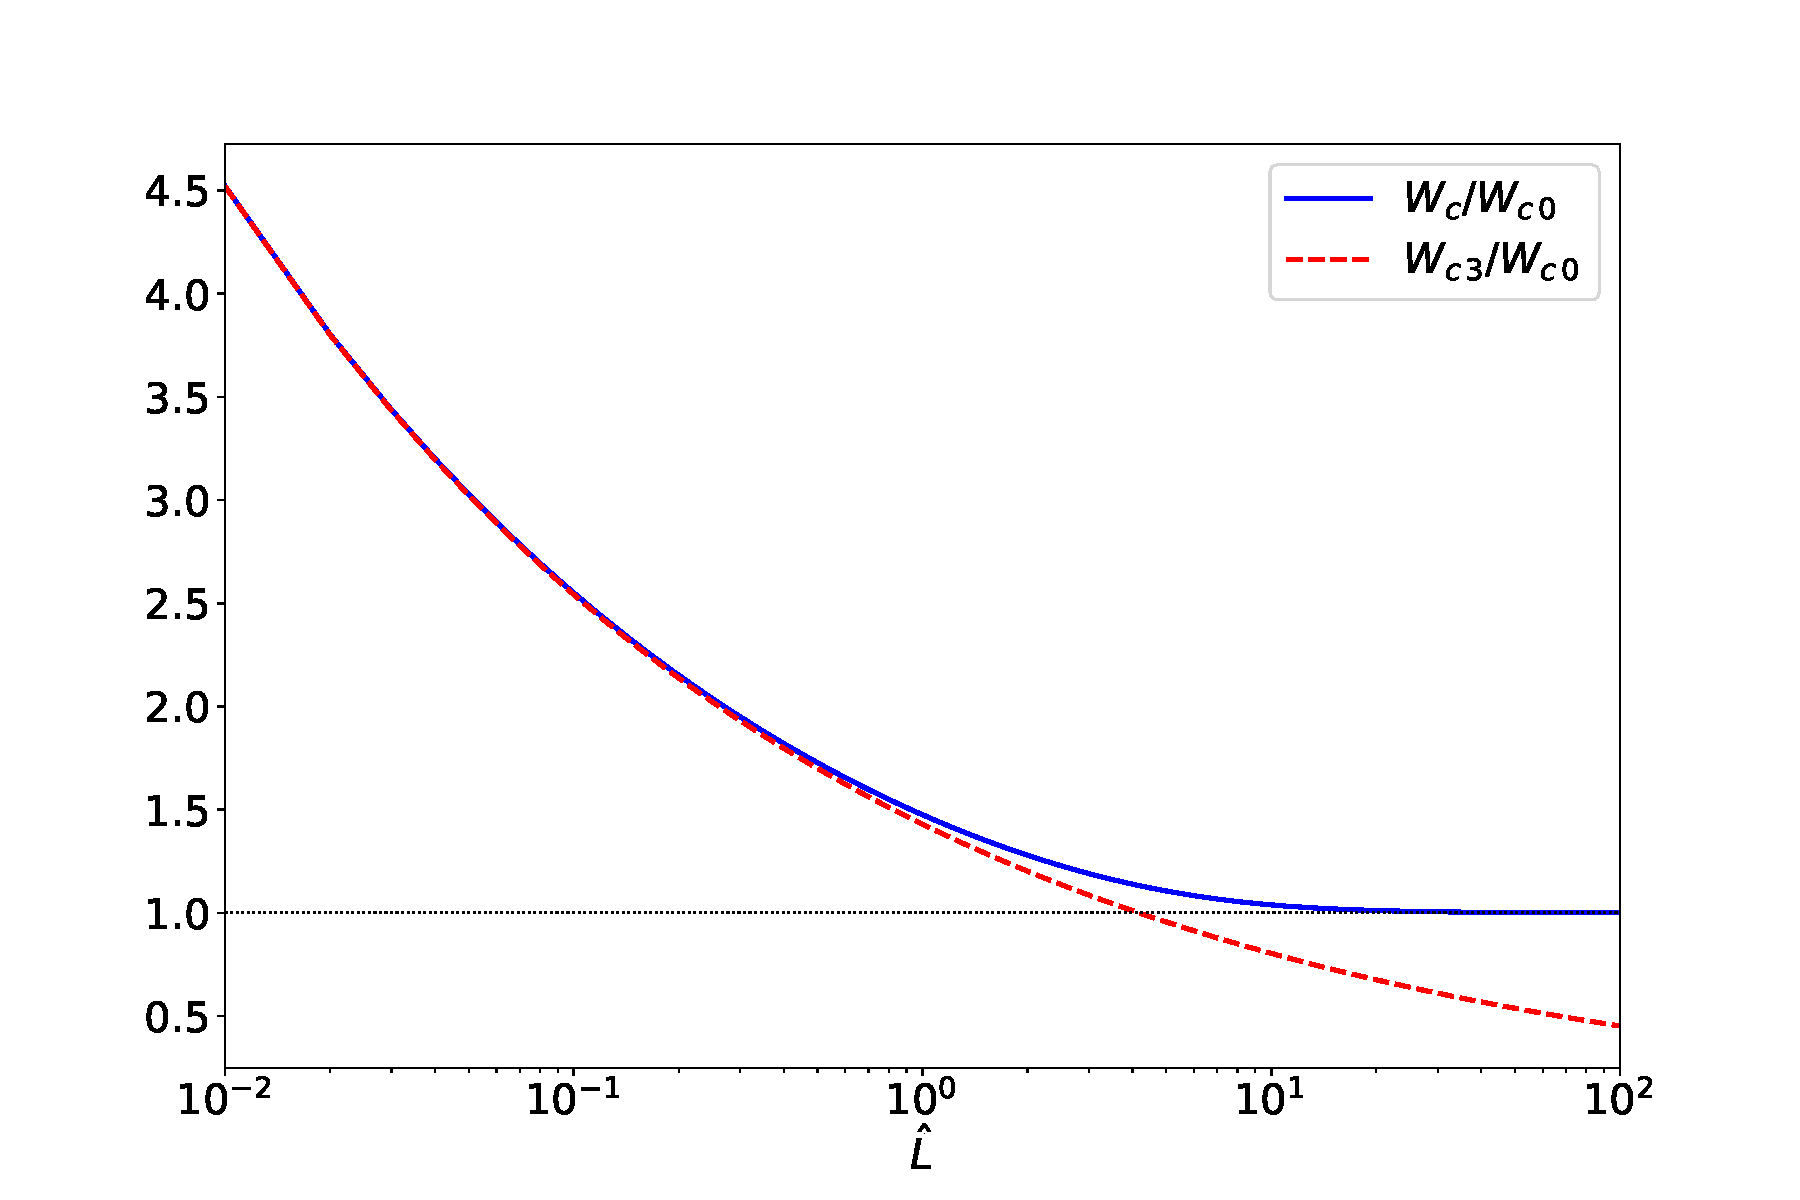
\includegraphics[width=1.0\textwidth]{zero.pdf}}
\caption{ Zero-frequency critical island width, $W_c$,  for electron temperature flattening, plotted as a function of the ratio of connection length to electron mean-free-path, $\hat{L}$. Also shown are the short and long mean-free-path limits, $W_{c\,0}$ and $W_{c\,3}$. Observe that $W_c\rightarrow  W_{c\,0}$ for $\hat{L}\gg 1$,   and $W_c\rightarrow W_{c\,3}$ for $\hat{L}\ll 1$. 
\label{fig3}}
\end{figure}

\begin{figure}
\centerline{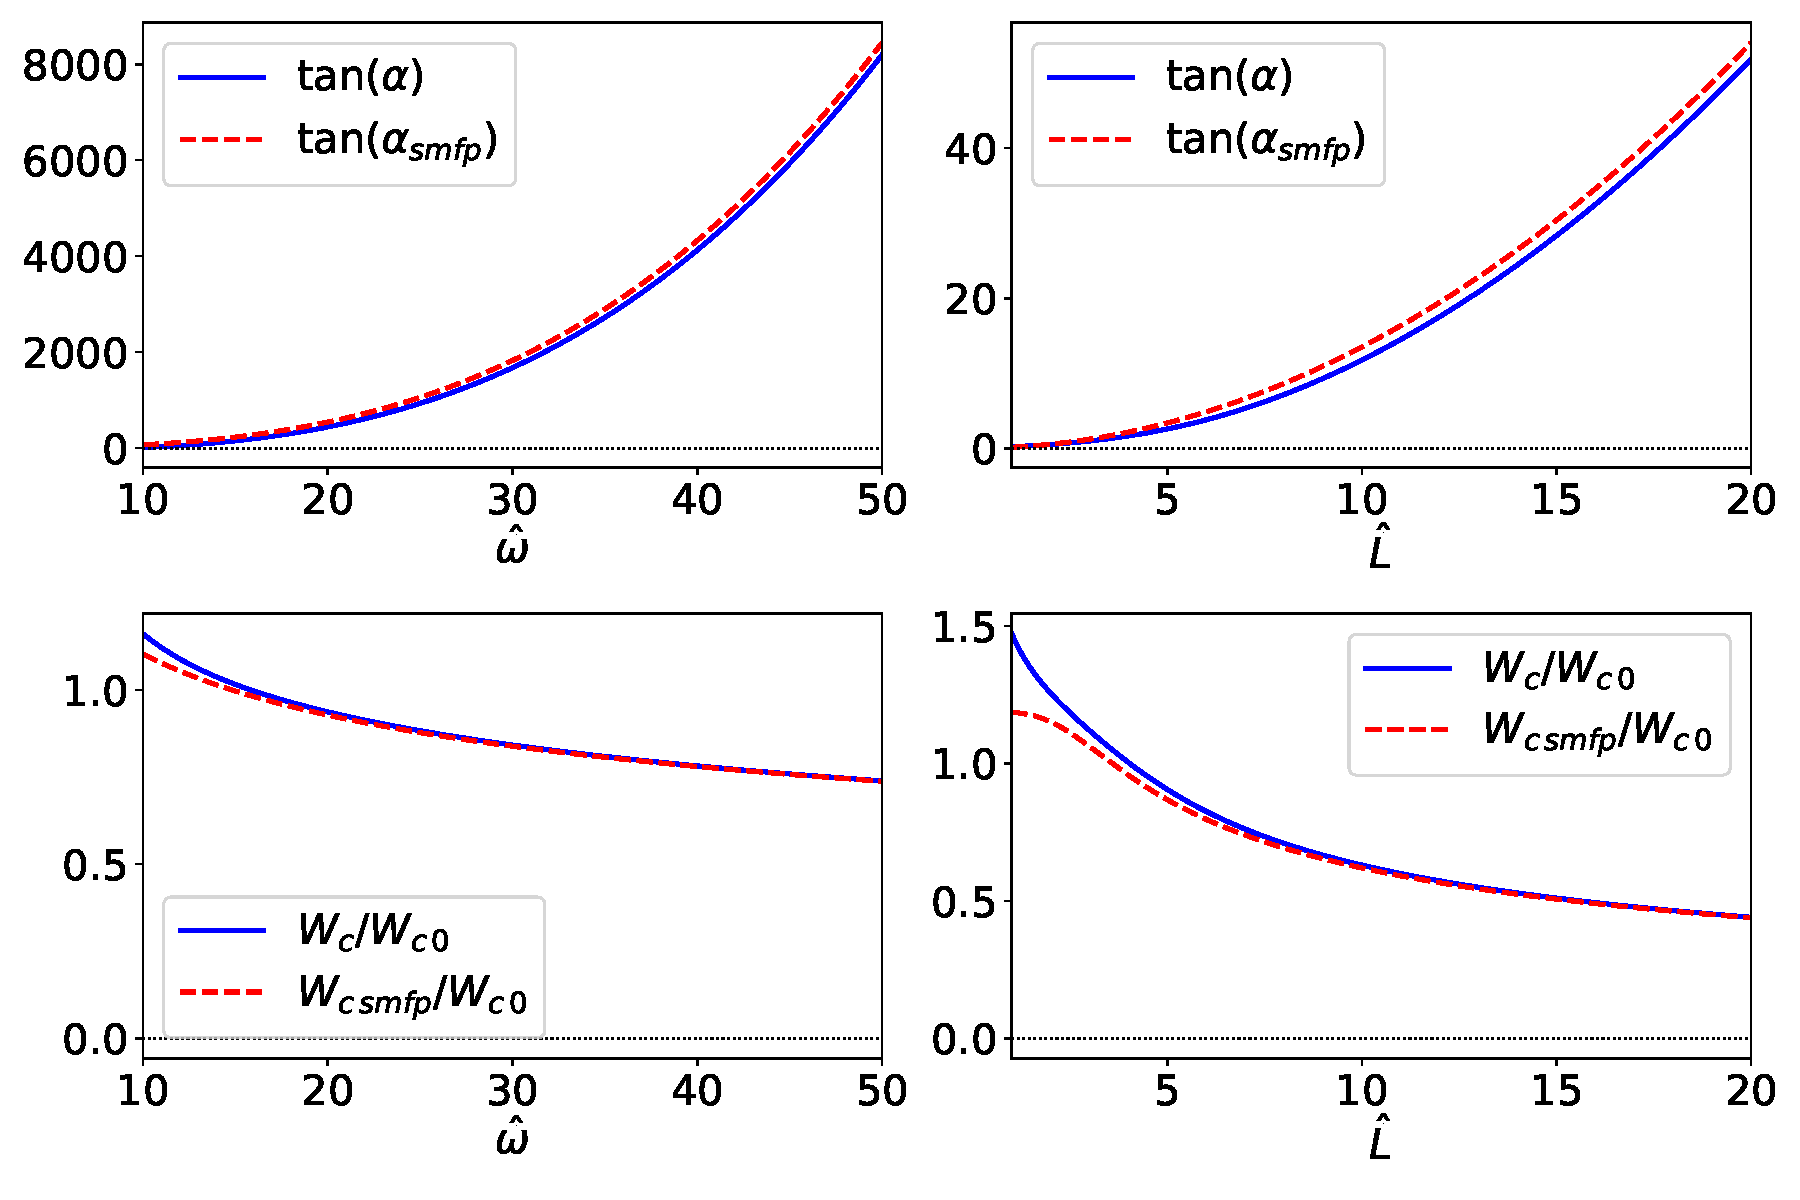
\includegraphics[width=1.0\textwidth]{smfp.pdf}}
\caption{Top-left panel: Tangent of the phase-lag, $\alpha$, plotted as a function of the normalized oscillation frequency, $\hat{\omega}$, for  $\hat{L}=1$. Also
shown is the tangent of the short mean-free-path phase-lag, $\alpha_{\rm smfp}$. Top-right panel: Same as top-left panel, except that
$\tan\alpha$ is plotted as a function of the normalized 
connection length, $\hat{L}$, for  $\hat{\omega}=1$.
Bottom-left panel: Normalized critical island width, $W_c/W_{c\,0}$,  plotted as a function of the normalized oscillation frequency, $\hat{\omega}$, for  $\hat{L}=1$. Also
shown is  short mean-free-path normalized island width, $W_{c\,{\rm smfp}}/W_{c\,0}$.  
Bottom-right panel: Same as the bottom-left panel, except that $W_c/W_{c\,0}$ is plotted as a function of the normalized 
connection length, $\hat{L}$, for  $\hat{\omega}=1$.
  \label{fig4}}
\end{figure}

\begin{figure}
\centerline{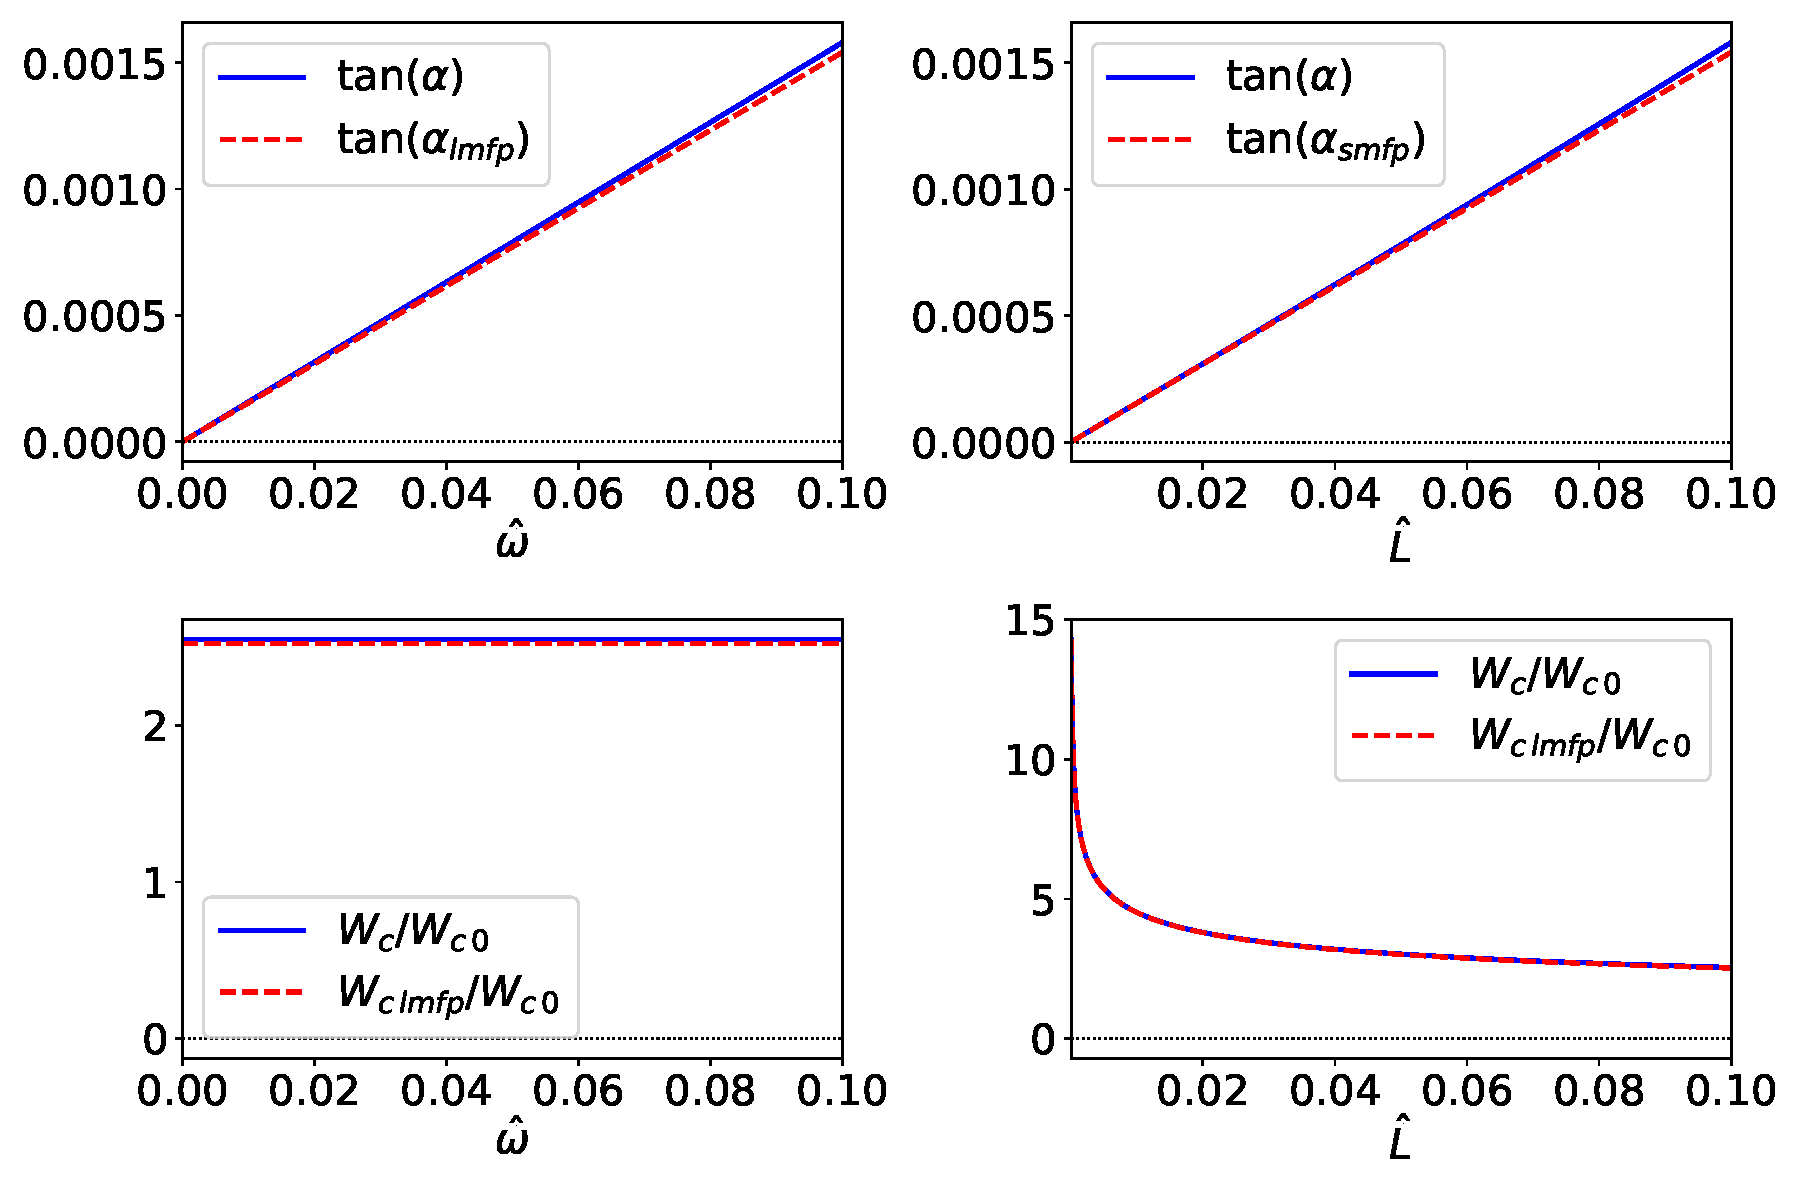
\includegraphics[width=1.0\textwidth]{lmfp.pdf}}
\caption{Top-left panel: Tangent of the phase-lag, $\alpha$, plotted as a function of the normalized oscillation frequency, $\hat{\omega}$, for  $\hat{L}=0.1$. Also
shown is the tangent of the long mean-free-path phase-lag, $\alpha_{\rm lmfp}$. Top-right panel: Same as top-left panel, except that
$\tan\alpha$ is plotted as a function of the normalized 
connection length, $\hat{L}$, for  $\hat{\omega}=0.1$.
Bottom-left panel: Normalized critical island width, $W_c/W_{c\,0}$,  plotted as a function of the normalized oscillation frequency, $\hat{\omega}$, for  $\hat{L}=0.1$. Also
shown is  long mean-free-path normalized island width, $W_{c\,{\rm lmfp}}/W_{c\,0}$.  
Bottom-right panel: Same as the bottom-left panel, except that $W_c/W_{c\,0}$ is plotted as a function of the normalized 
connection length, $\hat{L}$, for  $\hat{\omega}=0.1$.
  \label{fig5}}
\end{figure}

\end{document}